\documentclass[letter,12pt]{article}
\usepackage[utf8]{inputenc}
\usepackage{fullpage}
\usepackage{graphicx}
\usepackage{datetime}
\usepackage{indentfirst}

\newdateformat{mydate}{\THEDAY\space \shortmonthname[\THEMONTH] \THEYEAR}

\title{Switched LANs Lab Report}
\author{Sam Harkness}
\date{\mydate\today}

\begin{document}

%\maketitle

\begin{flushleft}
	\begin{tabular}{l l}
		To: & Prof. Richard Wolff \\
		From: & Sam Harkness \\
		Regarding: & TCP Lab Report \\
		Date: & \mydate\today
	\end{tabular}
\end{flushleft}



\begin{abstract}
	\noindent The objective of this lab is to demonstrate the congestion control algorithms implemented by the Transmission Control Protocol (TCP). The lab had us create 4 scenarios, all based on a base scenario of a server connected to a client, separated by an IP cloud:
	\begin{enumerate}
		\item NoDrop: The IP cloud will not drop any packets.
		\item Drop\_NoFast: The IP cloud will drop .05\% of packets, and will not recover from lost packets quickly.
		\item Drop\_Fast: The IP cloud will drop .05\% of packets, and will recover from lost packets quickly.
		\item Q4\_Drop\_Fast\_Buffer: The IP cloud will drop .05\% of packets,will recover from lost packets quickly, and has a much larger buffer window.
	\end{enumerate}
\end{abstract}

\section{Question 1:}
	The Segment Sequence Number remains unchanged because the server has not received an ACK, because of a dropped packet or the client's buffer is at capacity.  During this time, the server is not sending or receiving, so the connection is becoming less congested.

	\begin{figure}[h!]
		\centering
			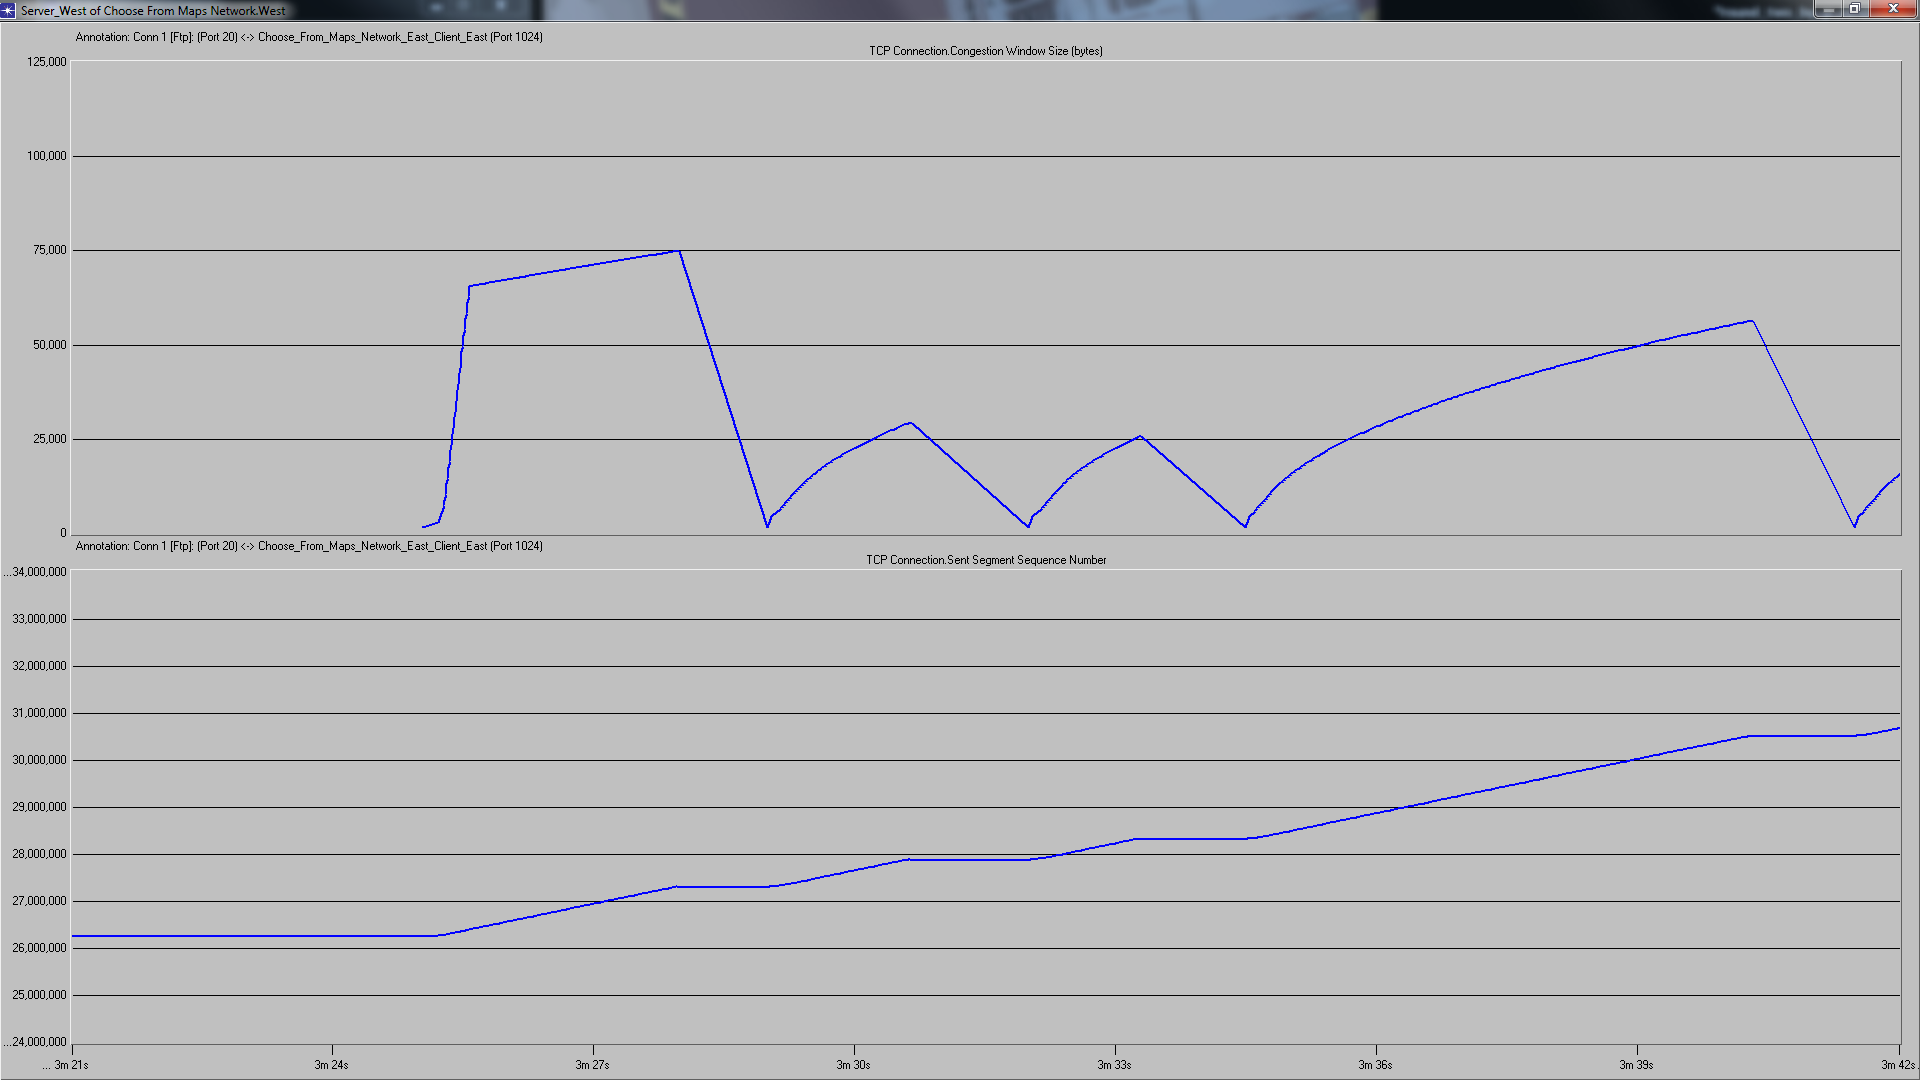
\includegraphics[width=.9\textwidth]{SequenceNum_vs_Congestion.png}
		\caption{Sequence Number vs Congestion}
		\label{SequencyNum_vs_Congestion}
	\end{figure}
	
\pagebreak

\section{Question 2:}
	The Drop\_NoFast scenario has the slowest growth in sequence numbers because the server must wait a timeout period after every packet is sent before it will resend a packet in the case of a drop.  The other reason it is the slowest is because it does not have the Fast Retransmit and Fast Recovery TCP options enabled.
	
	\begin{figure}[h!]
		\centering
			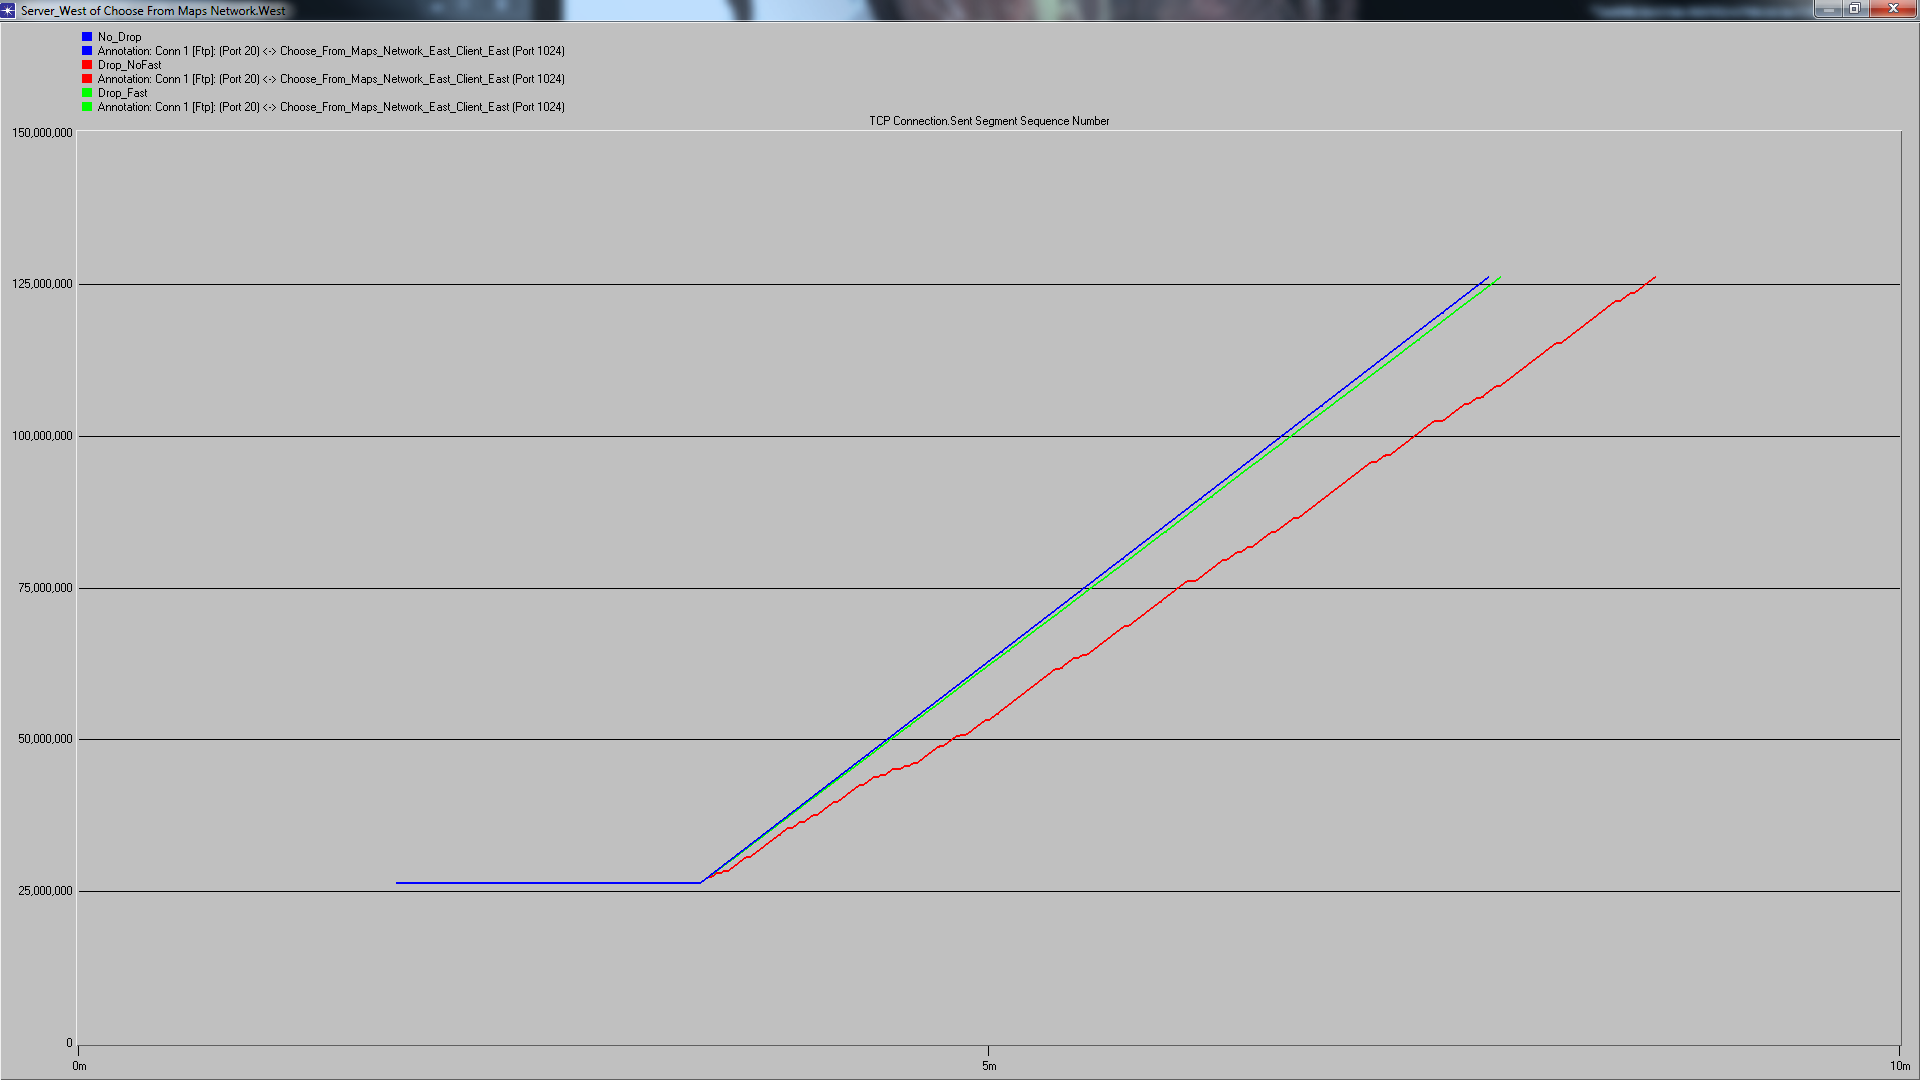
\includegraphics[width=.9\textwidth]{SequenceNum.png}
		\caption{Sequence Number of 3 Scenarios}
		\label{SequenceNum}
	\end{figure}
		
\pagebreak

\section{Question 3:}
	Sent Segment Number will always precede Received Segment ACK Number. When the Nth Received Segment ACK arrives, the server sends out the next Segment. The large pauses in both graphs correspond to a dropped packed.
	
	\begin{figure}[h!]
		\centering
			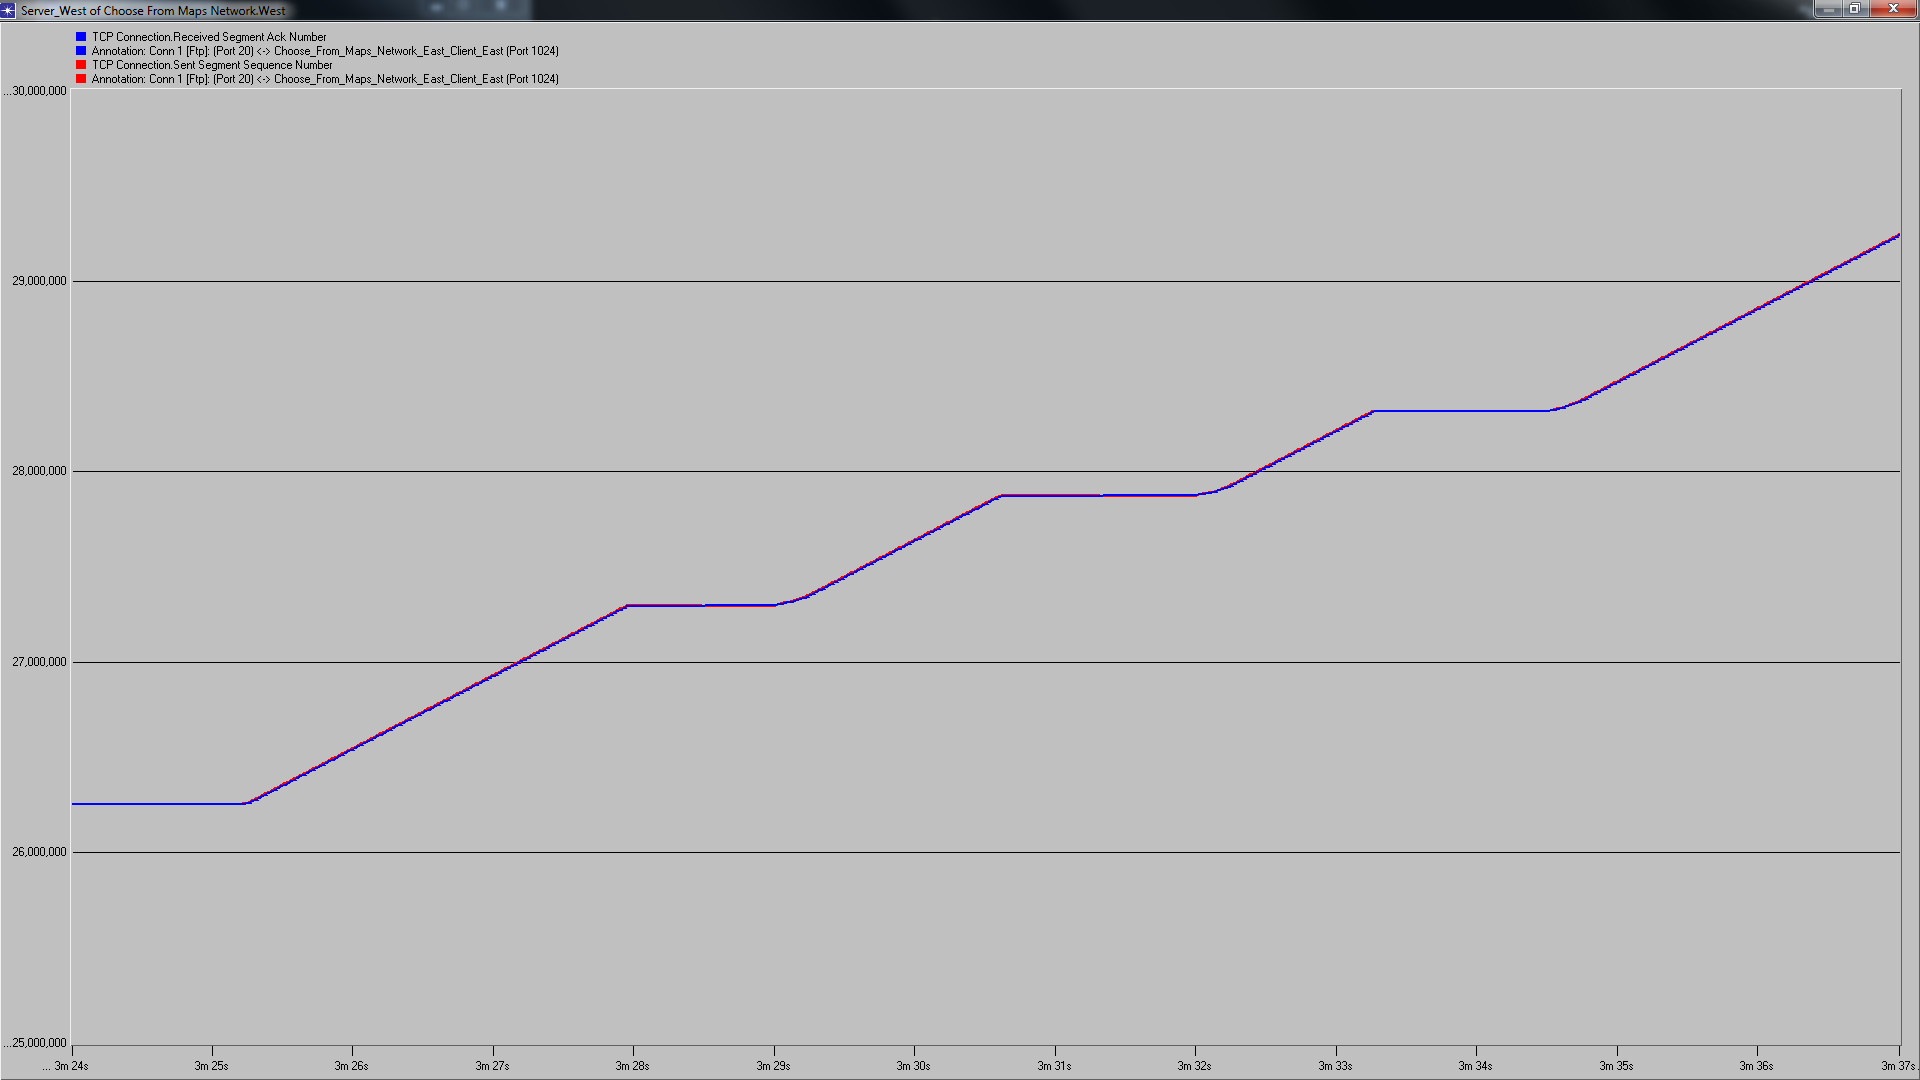
\includegraphics[width=.9\textwidth]{SequenceNum_vs_ACKNum.png}
		\caption{Sequence Number Sent vs Received ACK}
		\label{SequenceNum_vs_ACKNum}
	\end{figure}

\pagebreak

\section{Question 4:}
	Having a much larger buffer allows the client to receive much more data before it must stop sending ACKs to process the data.  This allows many more packets to be sent in a shorter timeframe, reducing the total length of the transmission, but increasing the amount of congestion.
	
	\begin{figure}[h!]
		\centering
			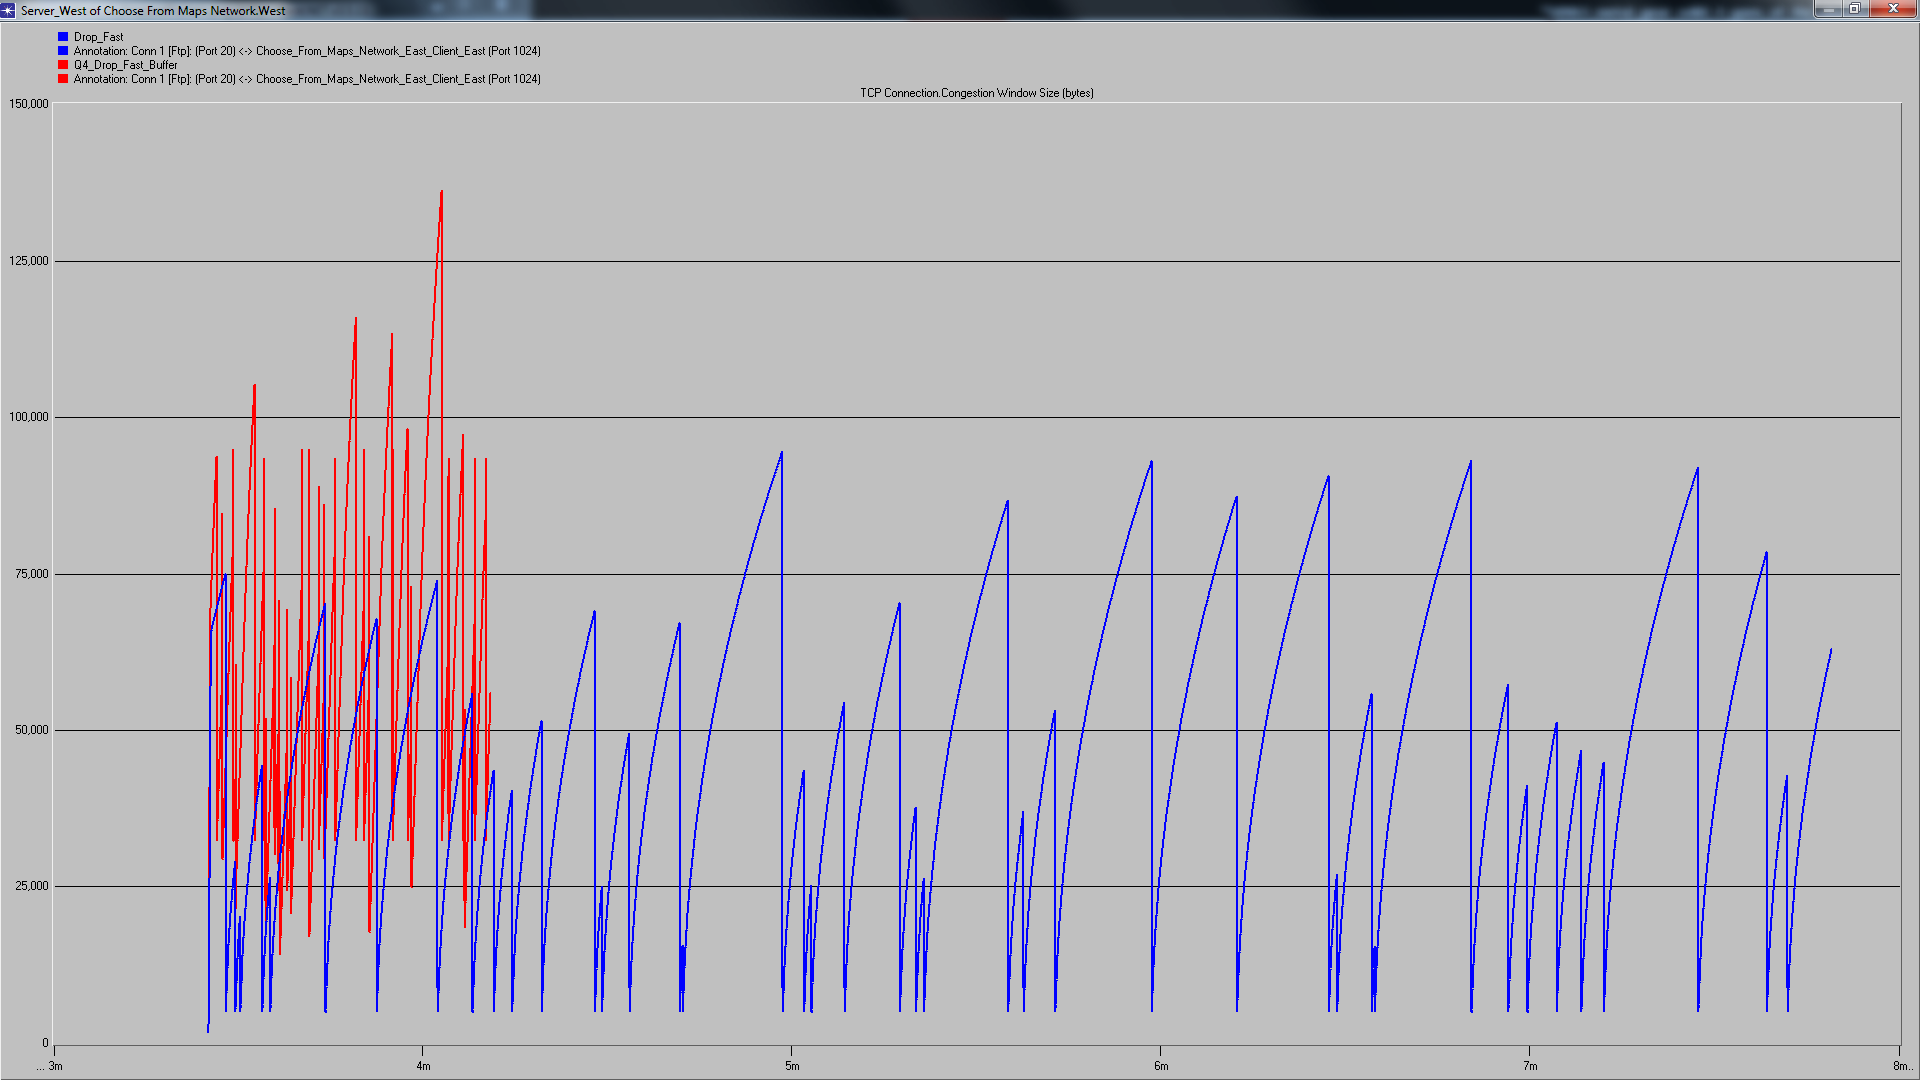
\includegraphics[width=.9\textwidth]{Congestion_Buffer.png}
		\caption{Congestion Window with and without an Increased Client Buffer}
		\label{Congestion_Buffer}
	\end{figure}
	
	
\end{document}
